% !TEX encoding = UTF-8 Unicode
\documentclass{scrartcl}
\usepackage{report}

\usepackage{fontspec}
\setmainhangulfont[Path=../fonts/,
  BoldFont={KoPub Batang Bold},
  ItalicFont={KoPub Dotum Light},
  BoldItalicFont={KoPub Dotum Bold}
]{KoPub Batang Light}
\setsanshangulfont[Path=../fonts/,
  BoldFont={KoPub Dotum Bold},
  ItalicFont={KoPub Batang Light},
  BoldItalicFont={KoPub Batang Bold}
]{KoPub Dotum Light}

\setkomafont{disposition}{\normalfont\bfseries}

% \cfoot{Page~\thepage~of~\pageref{LastPage}}

\begin{document}

\title{공간통계 보고서}
\subtitle{Burger Index: New city development index}
\author{이경원}
\affil{서울대학교 통계학과}
\date{\today}
\maketitle


\begin{abstract}
    본 보고서에서는 버거지수(Burger Index; BI)에 대해 알아보고, 이 값이 도시의 발전도를 나타낼 수 있는 지에 대해 공간통계학의 관점에서 살펴보고자 한다. 
\end{abstract}

\section{Introduction}   

현재, 전 세계 인구의 절반 이상은 도시지역에 거주하고 있다. 도시의 발전도는 인구밀집도와 높은 상관관계가 있으며 인구가 많은 큰 도시를 뜻하는 대도시(metropolitan)\가 정치, 경제, 문화의 중심이 되는 도시를 일컫는 데 사용되기도 한다. 도시발전지수(city development index)는 도시의 발전도를 의미하는 지표로 문화, 경제 등 다중공산성(multicolinearity)이 적다고 판단되는 여러 항목을 바탕으로 계산할 수 있다. 

버거지수(Burger Index; $BI$)는 2014년 한 트위터 유저(\autoref{fig:firstbi})에 의해 제안된 개념으로 $B,~M,~K,~L$을 각각 특정 도시 내의 버거킹, 맥도날드, KFC, 롯데리아 지점 수라고 했을 때 다음과 같이 정의된다
\begin{equation}\label{eqn:originbi}
    BI = \frac{B+M+K}{L}.
\end{equation}
해당 유저는 버거지수가 도시발전지수로 사용될 수 있다고 주장하였으며, 이후에도 \citet{jang2014} 등에 의해 탐색적 자료분석을 통한 정성적 확인이나 \autoref{fig:jangmap}와 같은 위상구조를 이용한 시각화가 이루어졌다. 반면에 실제 지리정보시스템(geographic information system; GIS)을 이용한 시각화나 회귀분석을 통한 정량적 분석은 거의 이루어지지 않았고, 버거지수의 구체적인 의미를 파악하는 데 어려움이 있었다.

\begin{figure}[!ht]
    \centering
    \begin{subfigure}[b]{0.6\textwidth}
        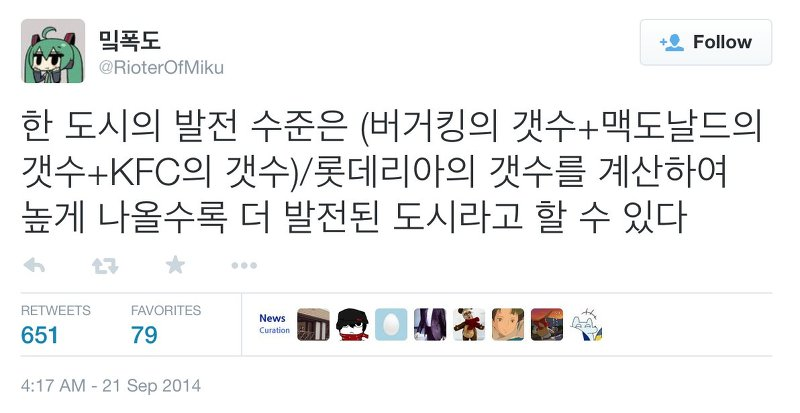
\includegraphics[width=\textwidth]{../figs/burgerindex.jpeg}
        \caption{최초로 제안된 버거지수}\label{fig:firstbi}
    \end{subfigure}~
    \begin{subfigure}[b]{0.3\textwidth}
        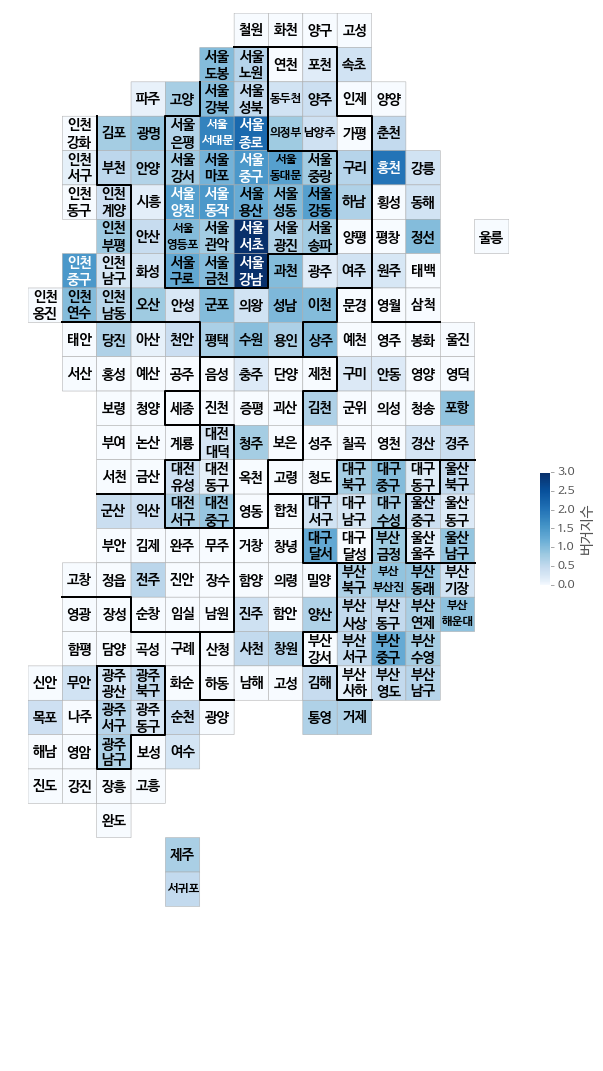
\includegraphics[width=\textwidth]{../figs/burgerindexmap.png}
        \caption{\citet{jang2014}, 버거지수 지도}\label{fig:jangmap}
    \end{subfigure}
    \caption{기존의 버거지수 관련 그림들}
\end{figure}

이번 보고서에서는 버거지수를 국내 지도에 시각화하고, 이 값이 실제로 도시발전지수에 사용될 수 있는지에 대해 살펴보고자 한다. \autoref{sec:data}에서는 자료 설명과 전처리 과정을, \autoref{sec:eda}에서는 전처리된 자료를 바탕으로 시각화 및 수치적 요약을 다룬다. \autoref{sec:sreg}에서는 공간회귀분석(spatial regression)\을 통해 버거지수가 실제로 어떤 의미를 가지고 있는지를 알아보고자 하며 그 결과와 논의를 각각 \autoref{sec:result}, \autoref{sec:con}에 정리하였다. 분석에 사용된 코드들은 github\footnote{\url{https://github.com/heleeos/BurgerIndex}}에 공개되어 있다.

\section{Data}\label{sec:data}

\subsection{Data Description}\label{subsec:data:desc}

\autoref{tbl:data:description}에 보고서에서 사용한 자료를 정리하였다. 

\begin{table}[ht]
    \centering
    \resizebox{0.8\textwidth}{!}{
	\begin{tabular}{c|p{13em}|c|c}
        \hline
        이름 & 설명 & 형태 & 출처 \\ \hline
		\texttt{burget/*} & 2019년 4월 기준 시군구별 패스트푸드 매장(버거킹, 맥도날드, KFC, 롯데리아, 맘스터치) 수 & xlsx(엑셀) & github\footnote{\url{https://github.com/idjoopal/BurgerIndex2019}} \\ \hline
		\texttt{pop/201903.xlsx} & 2019년 3월 기준 시군구별 주민등록 인구 자료 & xlsx(엑셀) & 국가통계포털\footnote{\url{http://kosis.kr/index/index.do}} \\ \hline
		\texttt{map/*} & 2019년 2월 기준 대한민국 시군구 단위 GIS 자료 & shp 등 & GIS DEVELOPER\footnote{\url{http://www.gisdeveloper.co.kr/?p=2332}} \\ \hline
    \end{tabular}
    }
	\caption{Data Description}\label{tbl:data:description}
\end{table}

저작권 등의 문제로 자료를 github에 업로드하지는 않았으며, 위의 출처에서 다운로드 받은 뒤 \texttt{data} 폴더 아래에 저장하여 사용하였다.

\subsection{Data Preprocessing}\label{subsec:data:preproc}

자료의 전처리는 R을 이용해 수행되었으며 대략적인 과정은 다음과 같다. 
\begin{enumerate}
    \item \texttt{xlsx} 파일들을 data frame의 형태로 불러온다.
    \item GIS 자료를 불러온 뒤 적절한 좌표계로 변환한다.
    \item 시군구별 패스트푸드 매장 수 자료들을 outer join으로 연결한다.
    \item GIS 자료에 패스트푸드 매장 수와 인구 자료를 left join으로 연결한다. 
    \item 각 시군구의 면적(area)와 중심점(centroid), 인구밀도(제곱킬로미터당 인구 수)를 계산한다.
    \item 각 시군구의 인접행렬(adjacency matrix; $W$)을 계산하여 저장한다.
\end{enumerate}

이때, 패스트푸드 매장 수 자료에서 일부 도시(특별시, 광역시를 제외한 시)의 구별 자료가 제공되어있지 않아 중소도시의 각 구별 매장 수는 전체 도시의 매장 수를 평균낸 값으로 할당하였다. GIS 자료의 전처리를 위한 코드는 서울대학교 공간통계 연구실의 자료를 활용하였다. 자료 전처리를 위한 소스코드는 github repository의 \texttt{scr/data\_preproc.R}에 제공되어 있으며, 전처리 결과의 spatial data frame \texttt{shp\_sig}\는 \texttt{rdata/shp\_sig.Rdata}에, 인접행렬 \texttt{W}\는 \texttt{rdata/nb\_sig\_mat.csv}에 저장하였다.

\section{Exploratory Data Analysis}\label{sec:eda}

이번 장에서는 버거지수와 관련된 탐색적 자료분석을 다룬다. \autoref{subsec:eda:vis}에서는 GIS 자료를 이용한 시각화를, \autoref{subsec:eda:numeric}에서는 각 설명변수들의 수치적 요약을 다룬다. 이때, \autoref{eqn:originbi}와 같이 버거지수를 계산하면 $L$ 값이 0일 때 값이 정의되지 않으므로, 연속성 수정계수를 도입하여 분모, 분자에 각각 1/2를 더한 다음과 같은 (수정된) 버거지수를 사용하였다
\begin{equation}\label{eqn:bi}
    BI_i = \frac{B_i+M_i+K_i+1/2}{L_i+1/2}.
\end{equation}

\subsection{Visualization}\label{subsec:eda:vis}

\texttt{ggplot2} 패키지와 GIS 자료를 이용해 각 자료를 시각화한 결과는 다음과 같다. \autoref{fig:fastfood}는 제곱킬로미터당 패스트푸드 매장 수를 브랜드별로 시각화한 것이다. 대부분의 패스트푸드 매장들이 수도권 지역에 몰려있다는 점과 롯데리아 매장이 다른 브랜드들에 비해 많은 점포수를 가지고 있다는 점을 확인할 수 있다. 

\autoref{fig:biandpopden}은 버거지수와 인구밀도를 시각화한 것인데, 일부 지역을 제외하면 버거지수와 인구밀도가 높은 지역이 광역시와 특별시 즉, 대도시임을 확인할 수 있다. \autoref{fig:jangmap}과 비교해보면 GIS 자료를 이용한 시각화가 현실적인 분포를 이해하는 데 유용함을 확인할 수 있다. \autoref{fig:jangmap}와 \autoref{fig:bi}의 버거지수 값의 차이는 계산하는 공식이 달라 발생한다. \citet{jang2014}은 (\ref{eqn:originbi})\로 버거지수를 계산하였으며 분모가 0인 시군구의 버거지수를 0으로 할당하였다.

\begin{figure}[!ht]
    \centering
    \begin{subfigure}[b]{0.475\textwidth}
        \centering
        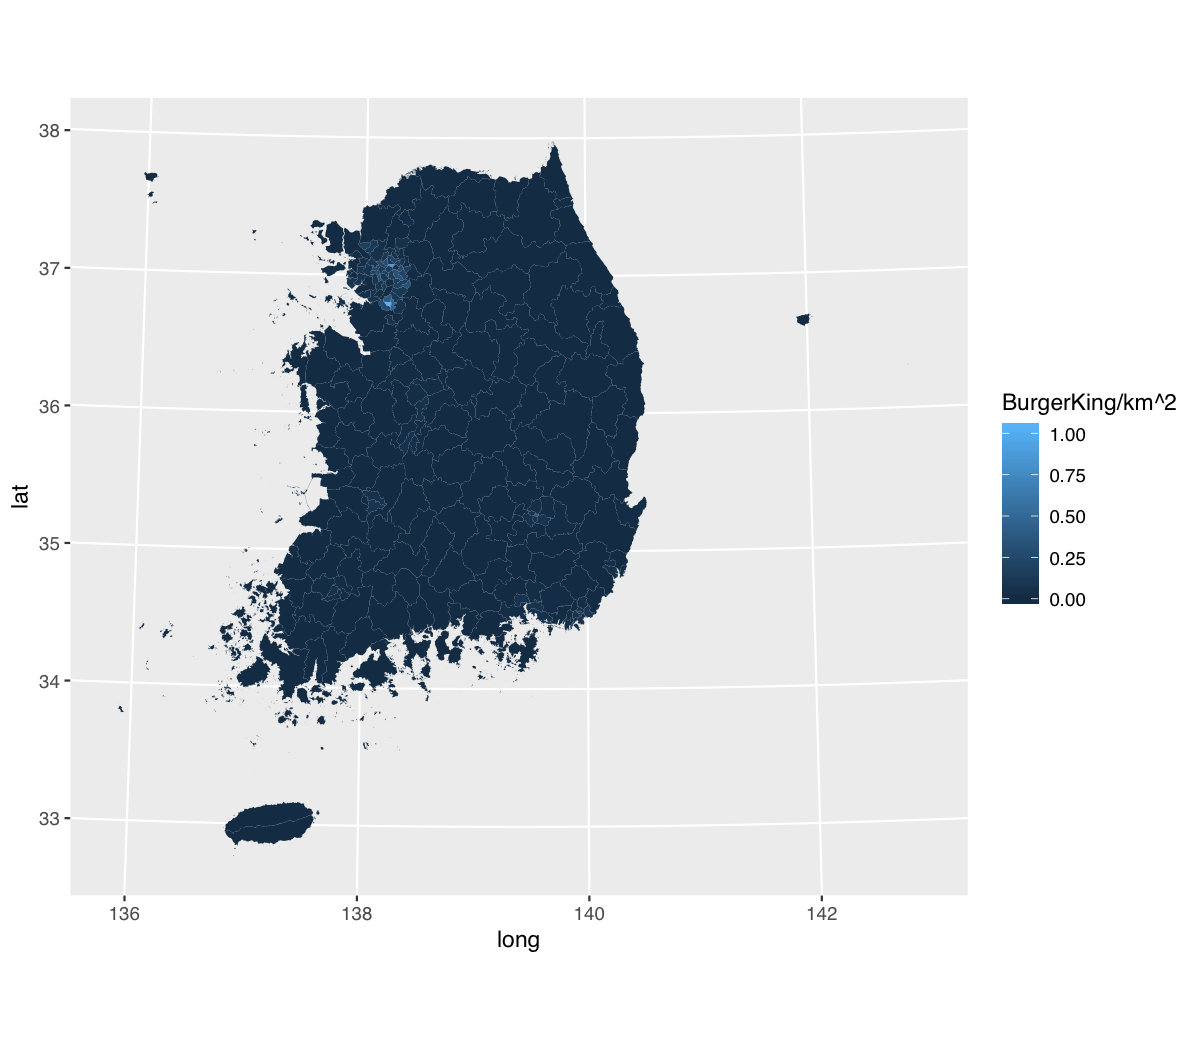
\includegraphics[width=\textwidth]{../figs/B_sig.png}
        \caption{버거킹}\label{fig:fastfood:B}
    \end{subfigure}
    \hfill
    \begin{subfigure}[b]{0.475\textwidth}  
        \centering 
        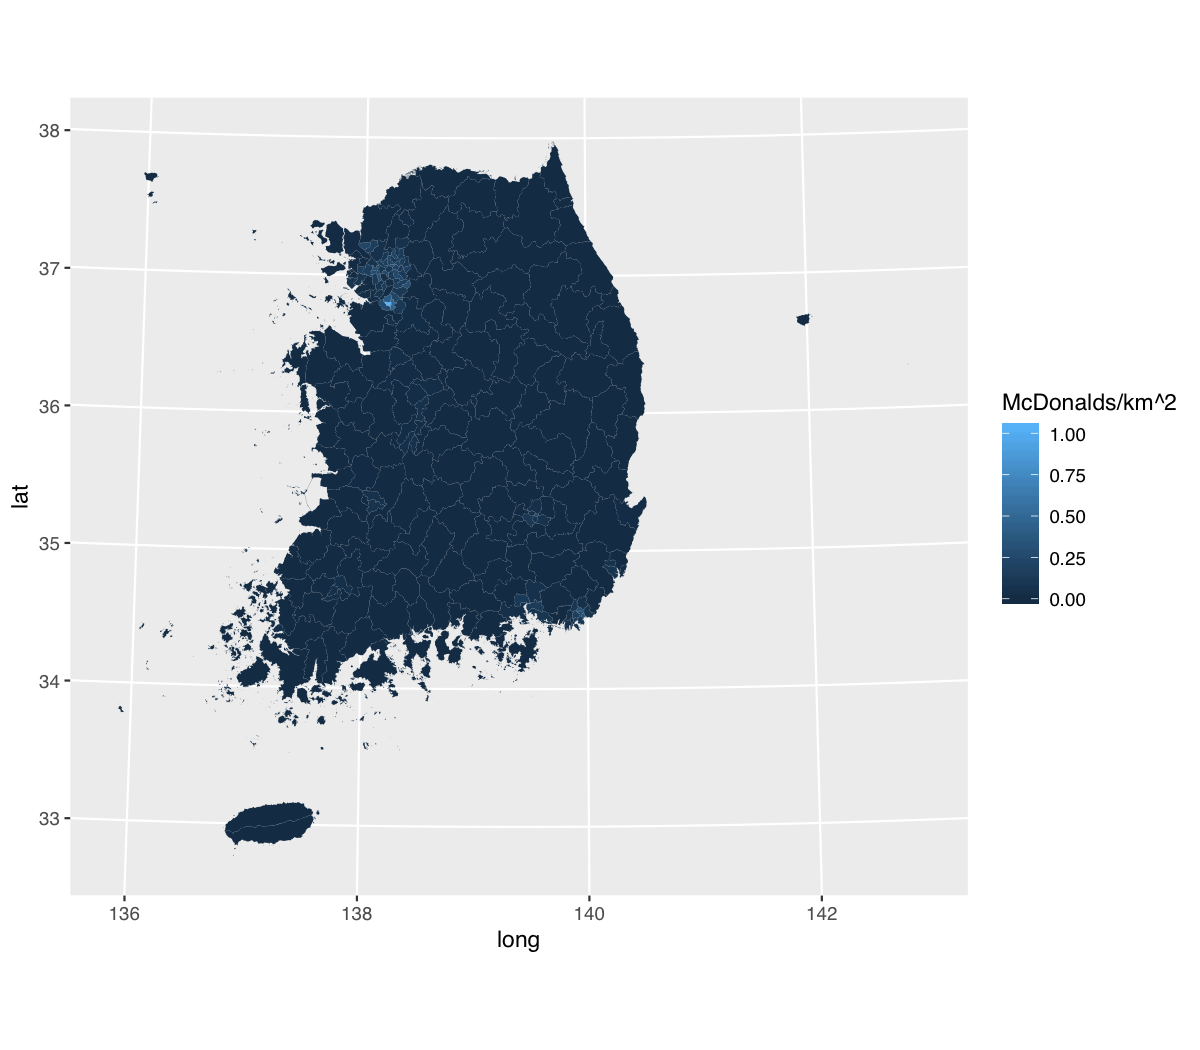
\includegraphics[width=\textwidth]{../figs/M_sig.png}
        \caption{맥도날드}\label{fig:fastfood:M}
    \end{subfigure}
    \vskip\baselineskip
    \begin{subfigure}[b]{0.475\textwidth}   
        \centering 
        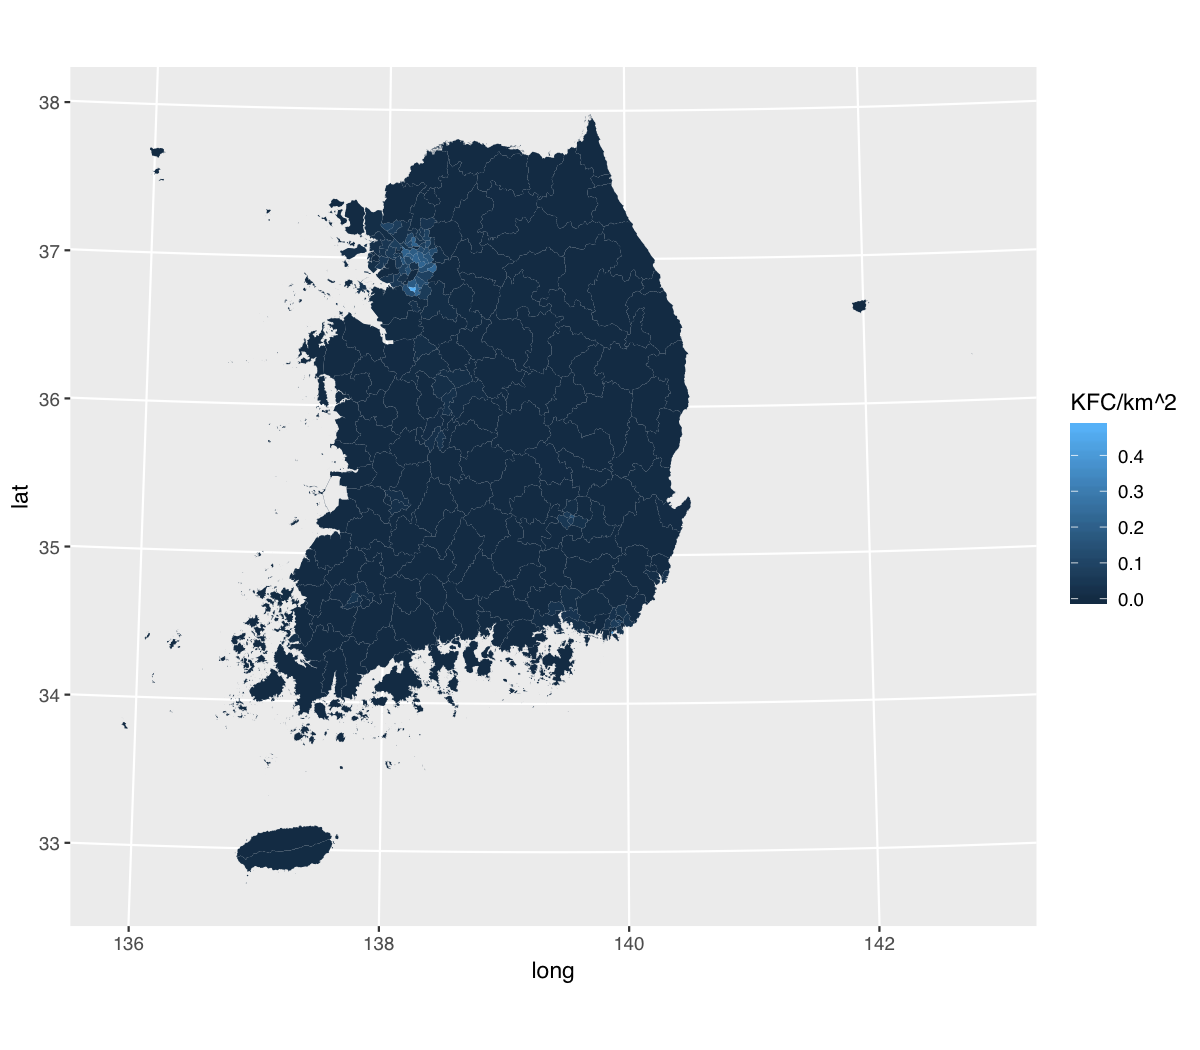
\includegraphics[width=\textwidth]{../figs/K_sig.png}
        \caption{KFC}\label{fig:fastfood:K}
    \end{subfigure}
    \quad
    \begin{subfigure}[b]{0.475\textwidth}   
        \centering 
        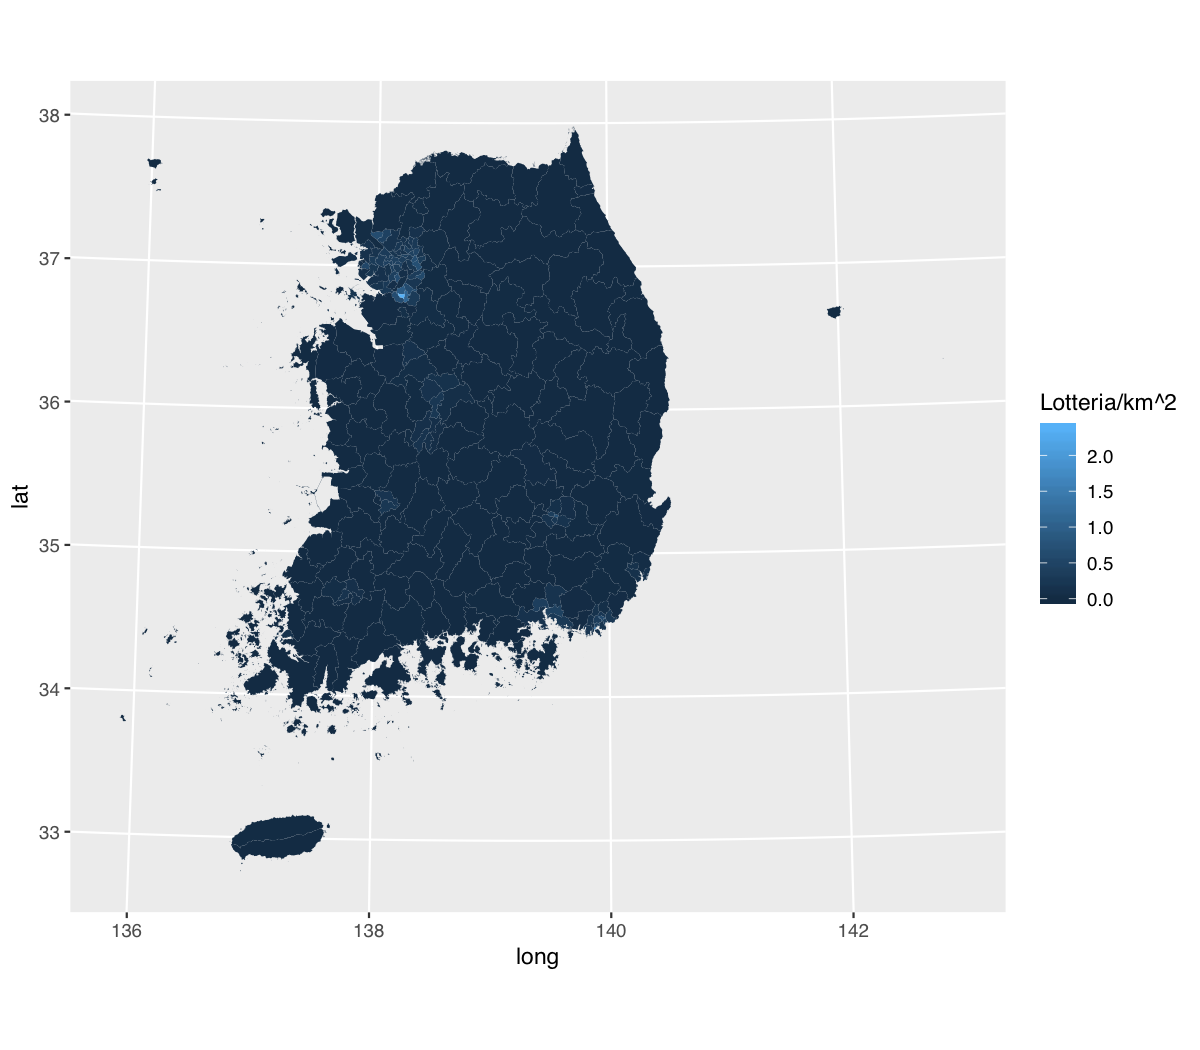
\includegraphics[width=\textwidth]{../figs/L_sig.png}
        \caption{롯데리아}\label{fig:fastfood:L}
    \end{subfigure}
    \caption{시군구별 제곱킬로미터당 패스트푸드 매장 수}
    \label{fig:fastfood}
\end{figure}   

\begin{figure}[!ht]
    \centering
    \begin{subfigure}[b]{0.475\textwidth}
        \centering
        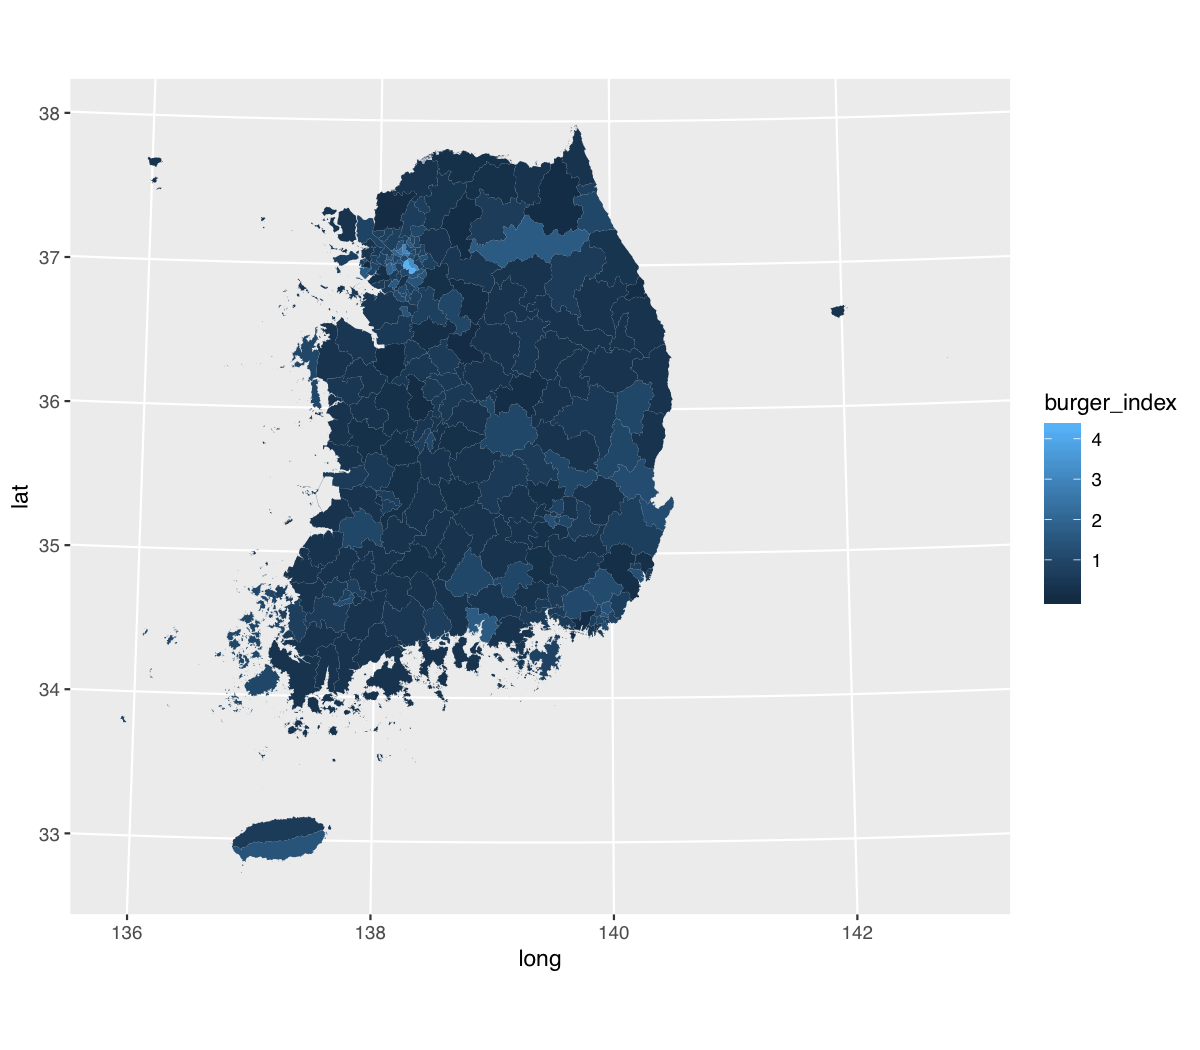
\includegraphics[width=\textwidth]{../figs/bi_sig.png}
        \caption{버거지수}\label{fig:bi}
    \end{subfigure}
    \hfill
    \begin{subfigure}[b]{0.475\textwidth}
        \centering
        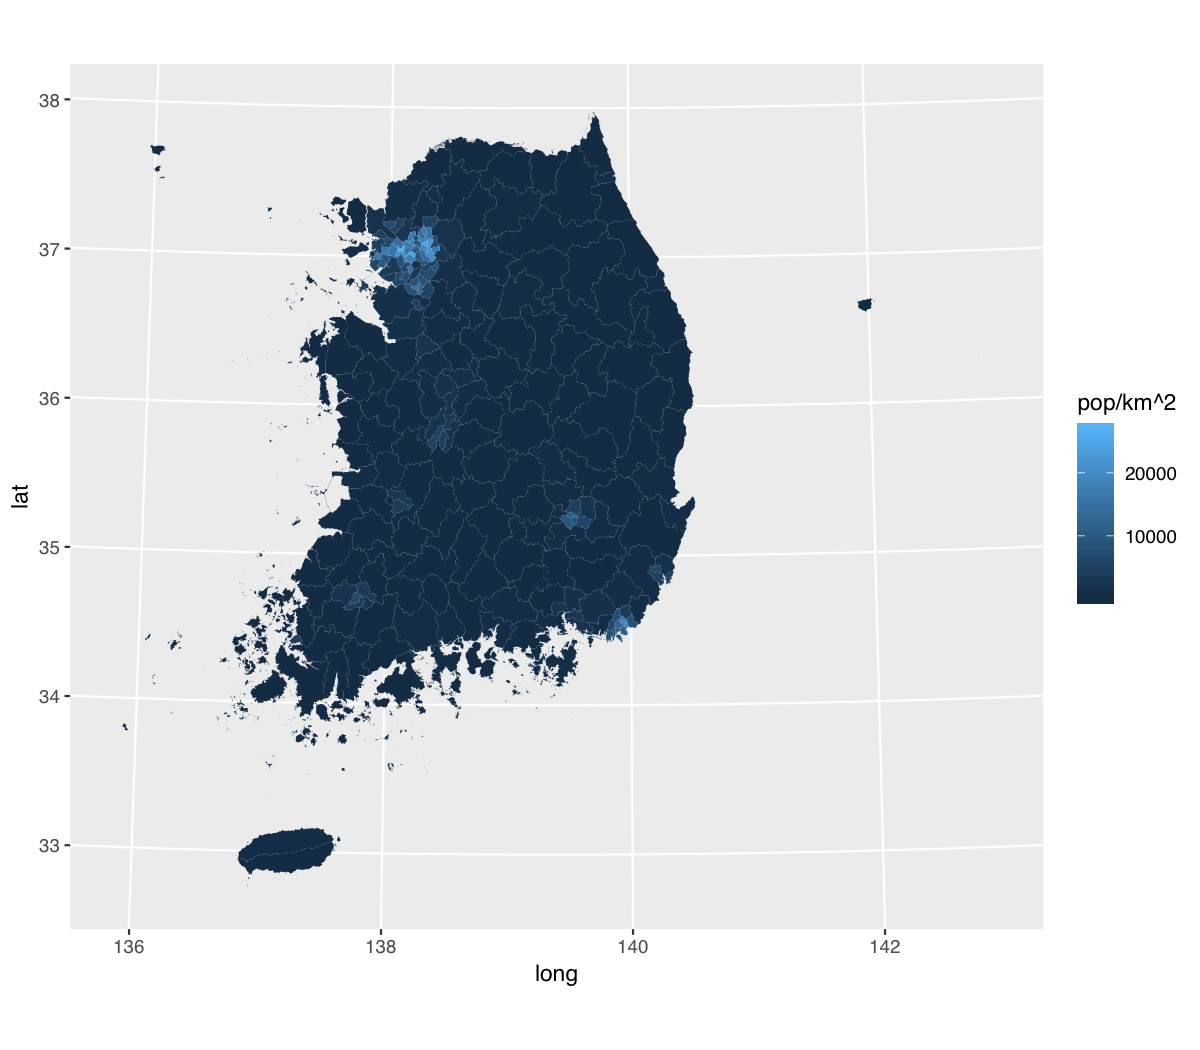
\includegraphics[width=\textwidth]{../figs/popden_sig.png}
        \caption{인구밀도}\label{fig:popden}
    \end{subfigure}
    \caption{버거지수와 인구밀도}\label{fig:biandpopden}
\end{figure}

\subsection{Numerical Analysis}\label{subsec:eda:numeric}

\autoref{tbl:summary}에 각 변수들의 요약통계량을 계산하였다. 앞서 예상한대로 롯데리아 매장 수가 다른 패스트푸드 브랜드에 비해 월등히 많다는 것과 지역별로 각 변수들의 표준편차가 매우 크다는 것을 확인할 수 있다. 분위수와 평균값을 확인해보면 자료의 분포가 왼쪽에 치우쳐져 있을 것이라 예상할 수 있다. 

\begin{table}[ht]
    \centering
    \begin{tabular}{c|rrrrrr}
      \hline
     & B & M & K & L & BI & pop\_density \\ 
     \hline
       mean & 1.94 & 2.26 & 1.11 & 7.48 & 0.68 & 4038.56 \\ 
       sd & 2.64 & 2.99 & 1.67 & 8.17 & 0.53 & 6083.81 \\ 
       Min. & 0.00 & 0.00 & 0.00 & 0.00 & 0.04 & 20.29 \\ 
       1st Qu. & 0.00 & 0.00 & 0.00 & 1.00 & 0.33 & 111.02 \\ 
       Median & 1.00 & 1.00 & 0.00 & 5.00 & 0.54 & 633.07 \\ 
       Mean & 1.94 & 2.26 & 1.11 & 7.48 & 0.68 & 4038.56 \\ 
       3rd Qu. & 3.00 & 4.00 & 2.00 & 10.00 & 0.90 & 6310.90 \\ 
       Max. & 13.00 & 13.00 & 10.00 & 34.00 & 4.27 & 27153.23 \\ 
    \hline
    \end{tabular}
    \caption{각 변수들의 요약통계량}\label{tbl:summary}
\end{table}

\autoref{fig:distribution}에 각 변수들의 분포를 나타내었다. 실제로 각 변수들은 왼쪽으로 치우쳐져 있으며 매장 수의 분포는 강한 양의 상관관계가 있다는 것을 확인할 수 있다. 또한, 버거지수와 인구밀도의 상관관계는 매장 수와 인구밀도의 상관관계보다 강한 것으로 확인된다. 
\begin{figure}
    \centering
    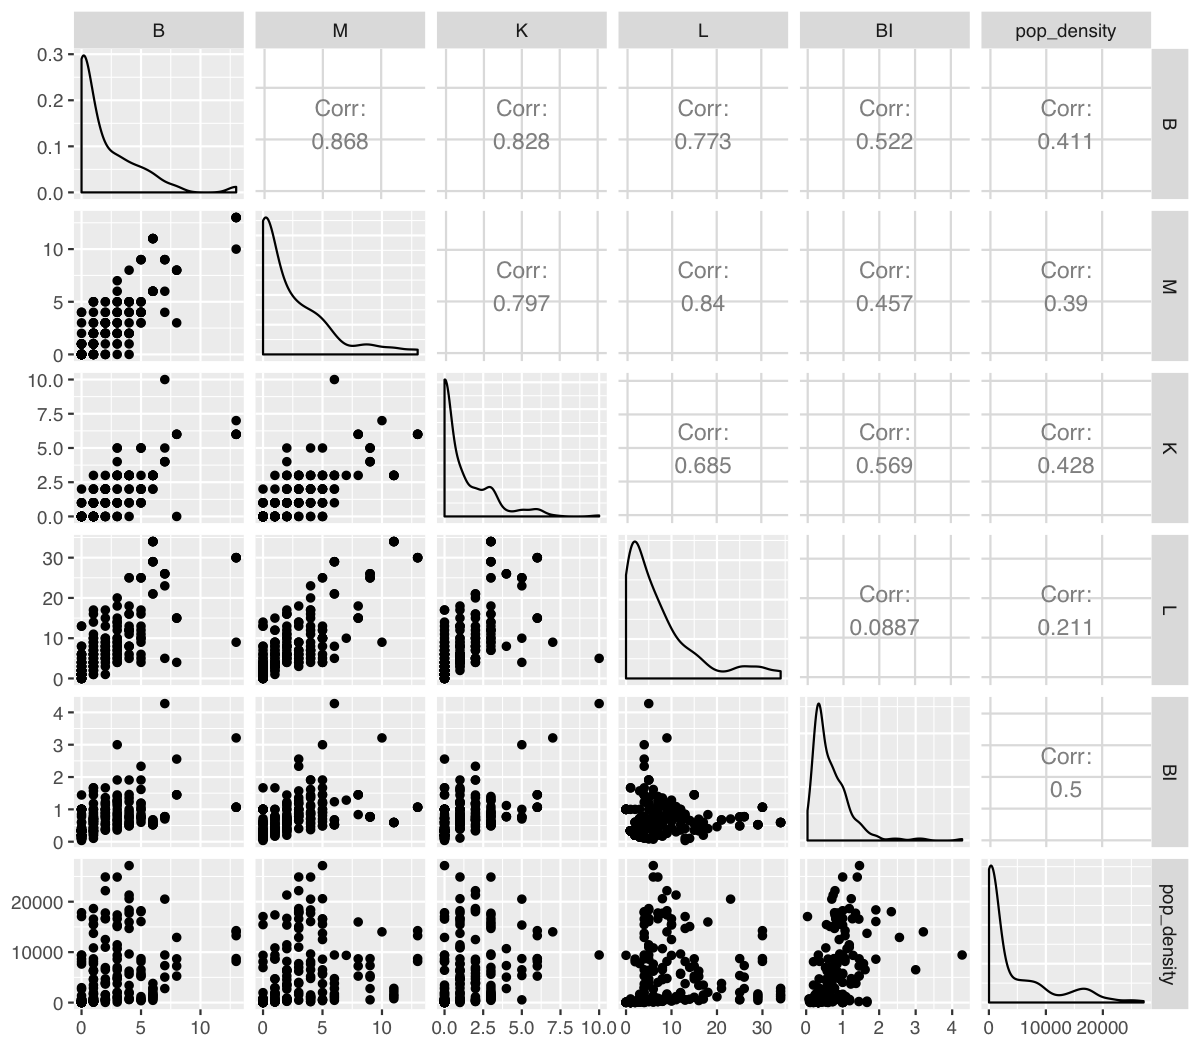
\includegraphics[width=0.7\textwidth]{../figs/dist_sig.png}
    \caption{각 변수들의 분포}\label{fig:distribution}
\end{figure}

\section{Spatial Regression Model}\label{sec:sreg}

\subsection{Model}\label{subsec:sreg:model}

본 보고서에서는 $i$번째 버거지수 $BI_i$를 다음과 같은 관계를 가진다고 가정하고 모형을 적합하였다.
\begin{equation}\label{eqn:sreg}
    \begin{gathered}
    BI_i = \frac{(B+M+K)_i+1/2}{L_i+1/2},\\
    BMK_i = (B+M+K)_i \sim \textrm{Poisson}(E_i \theta_i), \quad L_i \sim \textrm{Poisson}(E_i \phi_i), \\
    \log \theta_i = x_i^T \beta_1 + \epsilon_{1i}, \log \phi_i = x_i^T \beta_2 + \epsilon_{2i}, \\
    \epsilon_{ji} \sim \textrm{Proper CAR model}, \quad j=1,2. \\
    (\epsilon_{j.} = (\epsilon_{ji})_{i=1}^n \sim N(0,(\tau_j^2 (M-\gamma_j W))^{-1} ).)
    \end{gathered}
\end{equation}
여기서 $E_i$는 면적/100을 사용하였으며 $x_i = (1, \texttt{cen\_long}_i, \texttt{cen\_lat}_i, \texttt{pop\_density}_i)^T$, 즉, 설명변수로 시군구의 중심점의 위치와 인구밀도를 사용하였다. 회귀계수의 해석을 위해 각 설명변수는 표준화하여 사용하였다. 모수 $\beta_j,~\tau_j,~\gamma_j$를 추정하기 위한 사전분포로는 각각 $N(0, 10^2),~\textrm{Gamma}(0.1, 0.1),~U(0,1)$을 사용하였다. 표본추출은 Hamiltonian MCMC를 사용하였으며, \texttt{src/poisson\_proper\_car.*} 파일에 표본추출을 위한 코드가 저장되어있다. 4개의 chain, 1,000개의 표본을 추출하였으며 이중 500개의 표본은 warm-up sample로 사용되었다. 

모형을 적합하는 과정에서 오류가 발생했는데, 이것은 $W$의 특정 행의 모든 성분들이 0으로 계산되는 것에서 기인했다. 확인 결과 속초, 부천 등 실제로는 인접한 지역이 존재하는 위치이나 GIS 자료의 문제로 인접한 지역이 존재하지 않는 자료처럼 계산되고 있었다. 이 문제를 회피하기 위해 모든 성분이 0으로 계산되는 $W$의 행의 대각성분에 1을 더해주었다.

표본 추출에는 iMac(Intel Kaby Lake (7th) 3.5GHz Quad core i5-7600, 16GB RAM) 기준 chain 당 20분 정도의 시간이 소요되었다. 추출된 표본들(\texttt{bmk\_fit}, \texttt{l\_fit})\을 \texttt{rdata/sreg.Rdata} 파일에 저장하였다.

\section{Results}\label{sec:result}

이번 장에서는 회귀모형 (\ref{eqn:sreg})에서 추출된 사후표본과 예측치에 대한 해석을 다룬다.

\subsection{Estimation}

\autoref{fig:traceplot}은 추출된 표본들의 trace plot을 그린 것이다. 회색 음영부분은 warm-up에 사용된 표본들로 모든 회귀계수가 빠르게, 잘 수렴함을 확인할 수 있다. \autoref{fig:denseplot}은 추출된 표본들로 추정한 사후분포를 그린 것이다. $BMK$와 $L$ 모두에서 인구밀도(\texttt{beta[4]})가 강한 영향을 미치고 있음을 확인할 수 있다. 또한, $\gamma$이 모두 1에 가깝게 추정되었으므로 이 모형은 intrinsic CAR에 가까운 모형이라 말할 수 있다.

\begin{figure}[!ht]
    \centering
    \begin{subfigure}[b]{0.9\textwidth}
        \centering
        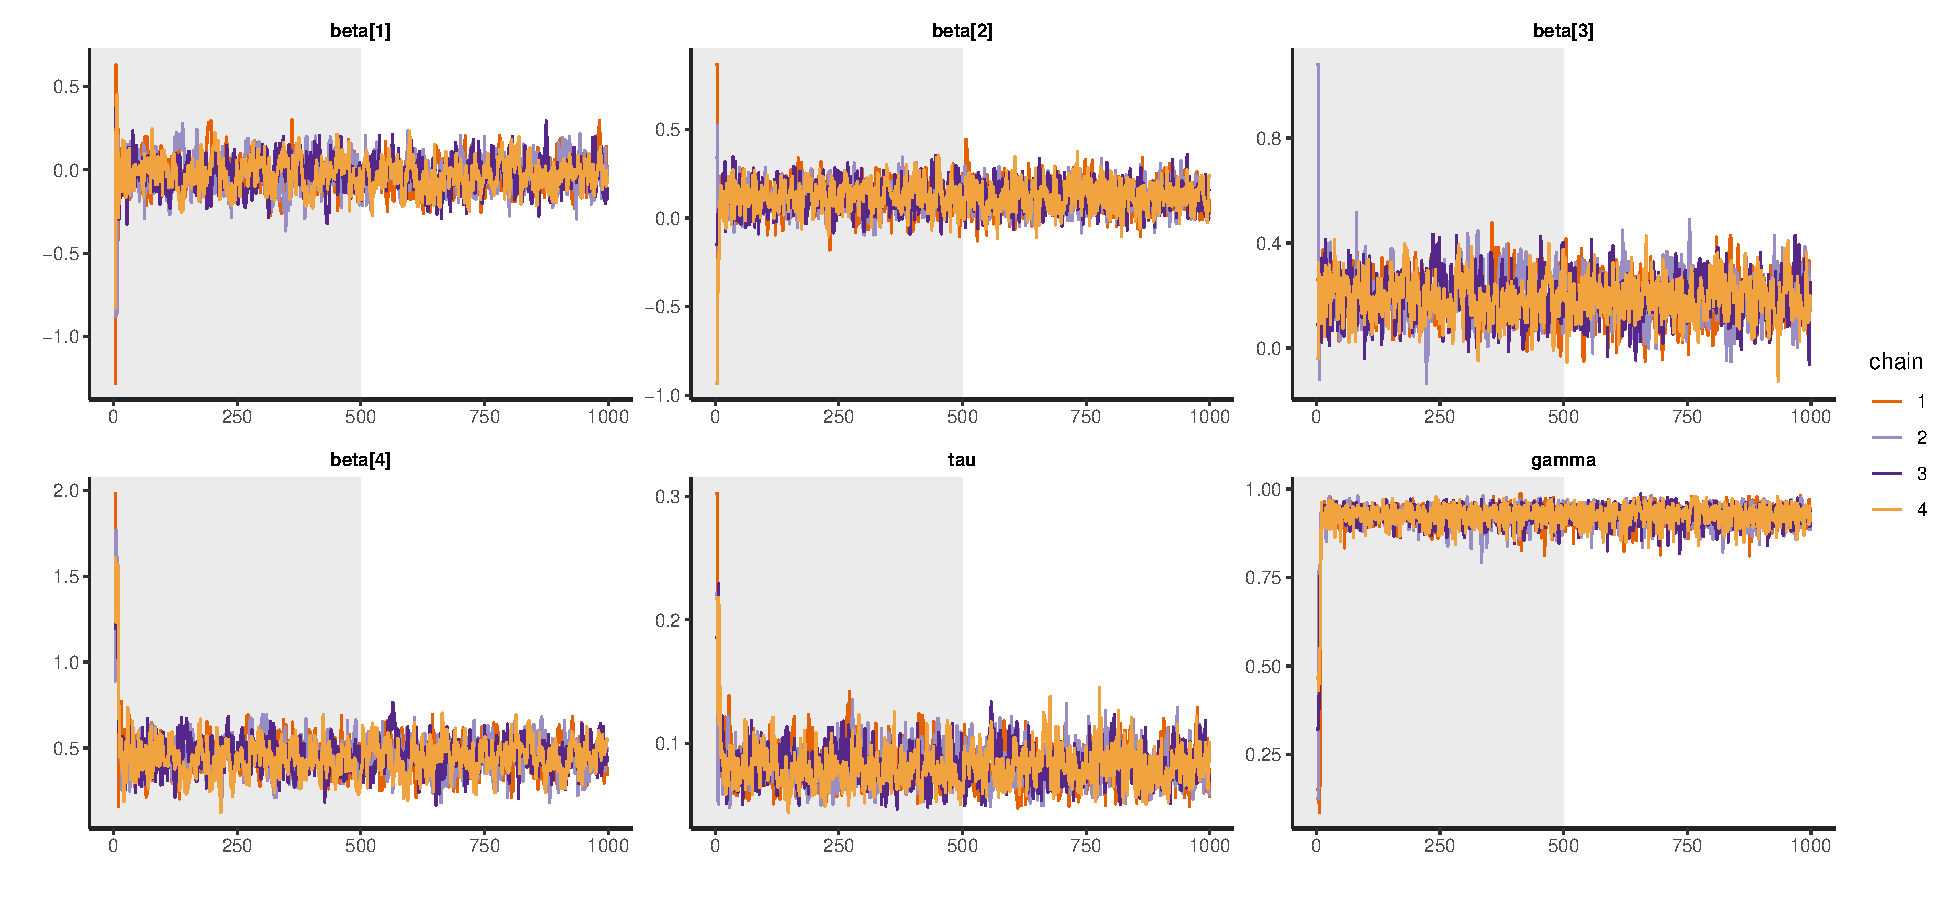
\includegraphics[width=\textwidth]{../figs/mcmc/bmk_trace.pdf}
        \caption{Traceplot of $\beta_1,~\tau_1,~\gamma_1$}\label{fig:traceplot:bmk}
    \end{subfigure}
    \vskip\baselineskip
    % \hfill
    \begin{subfigure}[b]{0.9\textwidth}   
        \centering 
        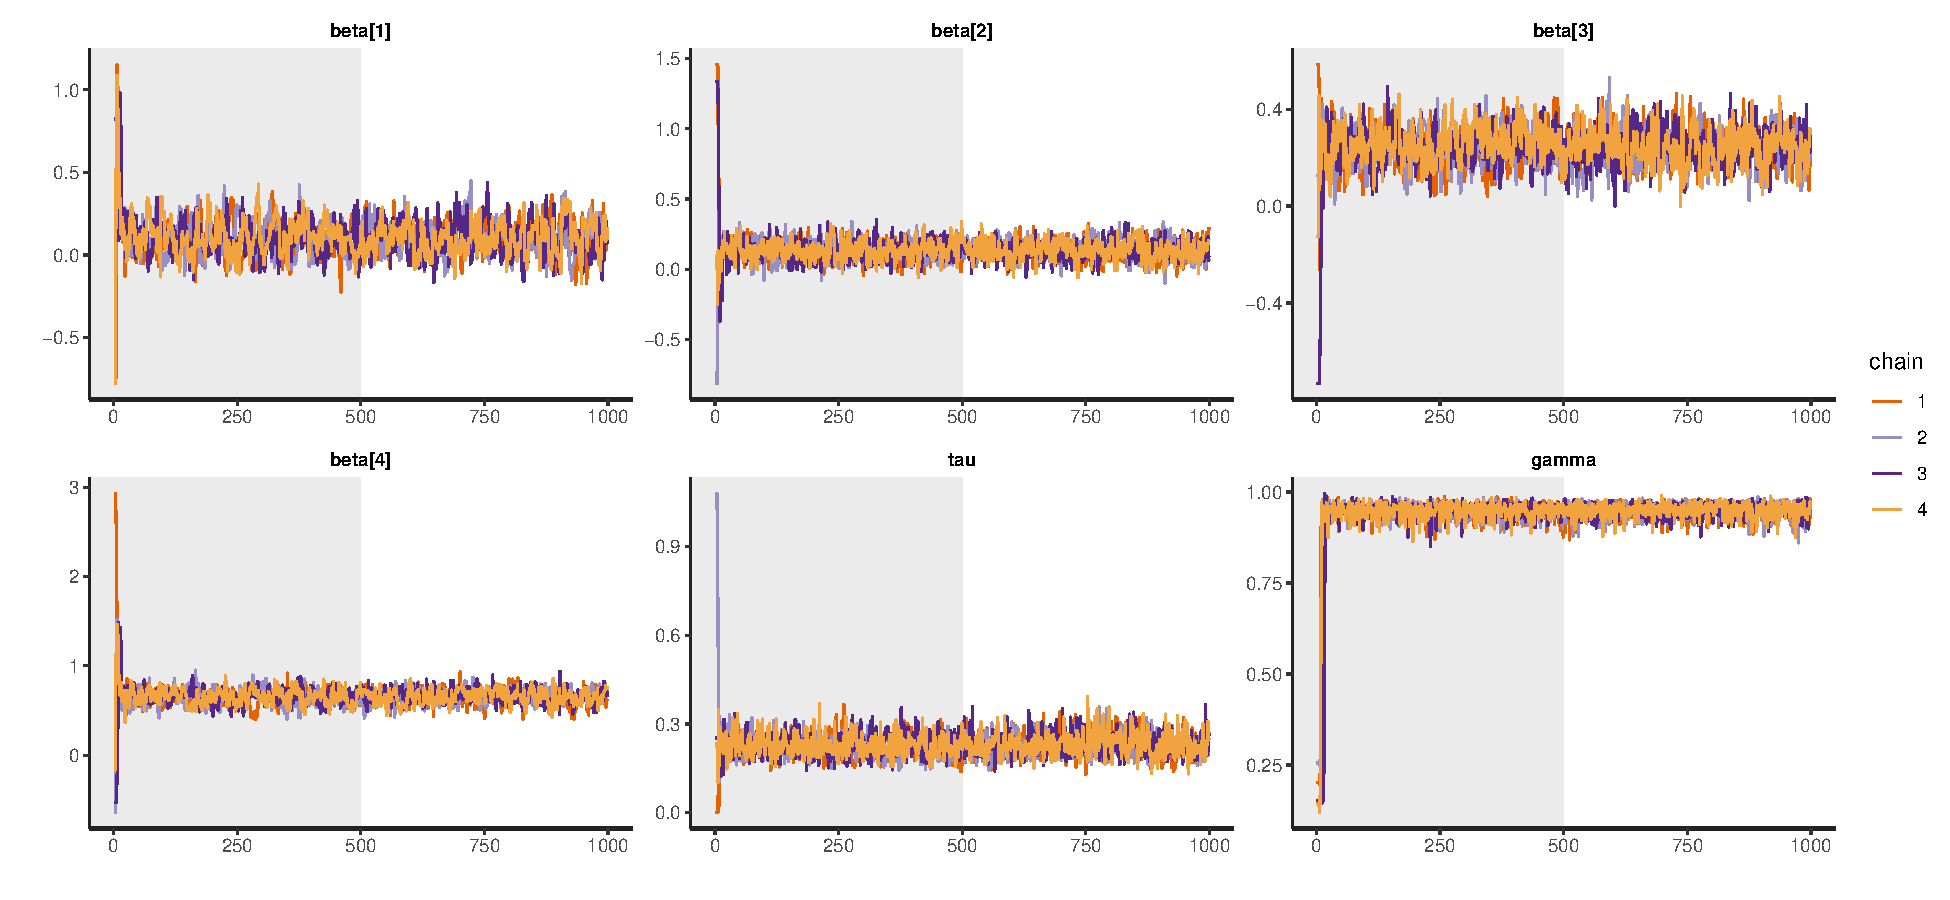
\includegraphics[width=\textwidth]{../figs/mcmc/l_trace.pdf}
        \caption{Traceplot of $\beta_2,~\tau_2,~\gamma_2$}\label{fig:traceplot:l}
    \end{subfigure}
    \caption{Trace plot of MCMC samples}
    \label{fig:traceplot}
\end{figure}   

\begin{figure}[!ht]
    \centering
    \begin{subfigure}[b]{0.45\textwidth}
        \centering
        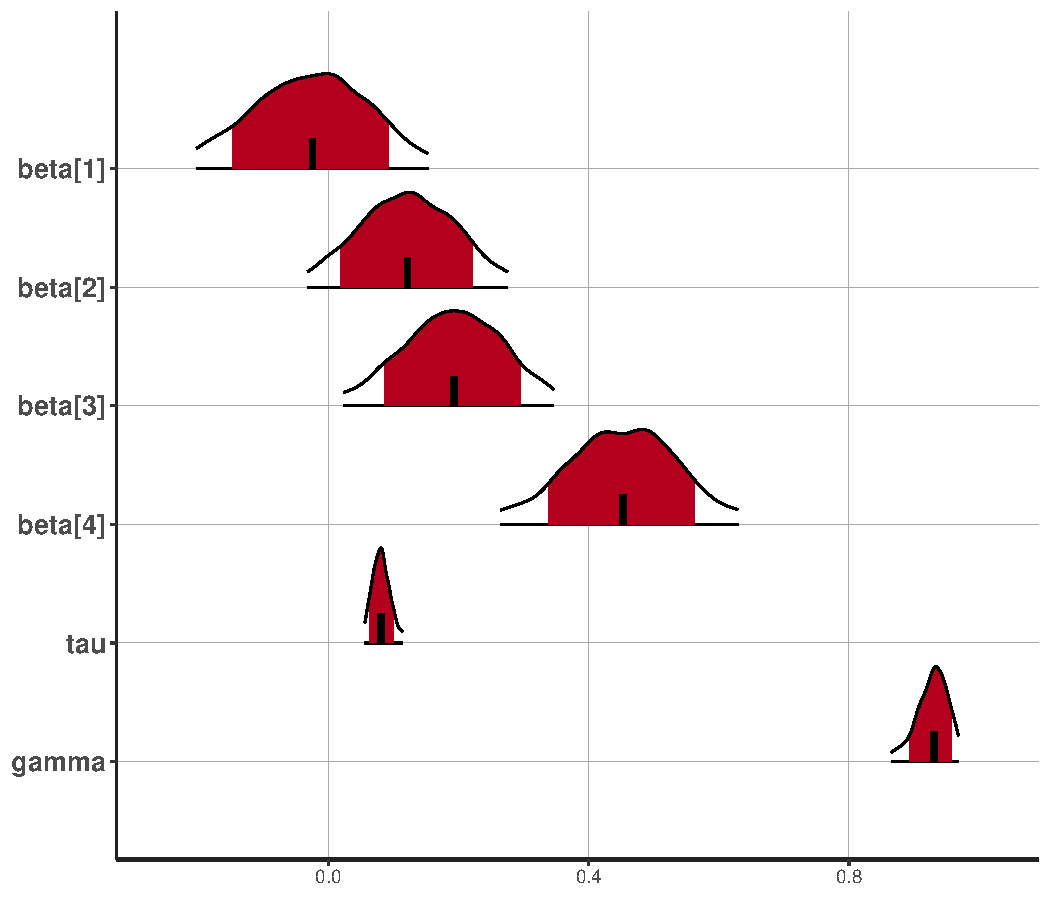
\includegraphics[width=\textwidth]{../figs/mcmc/bmk_dens.pdf}
        \caption{Estimated posterior of $\beta_1,~\tau_1,~\gamma_1$}\label{fig:denseplot:bmk}
    \end{subfigure}
    % \vskip\baselineskip
    \hfill
    \begin{subfigure}[b]{0.45\textwidth}   
        \centering 
        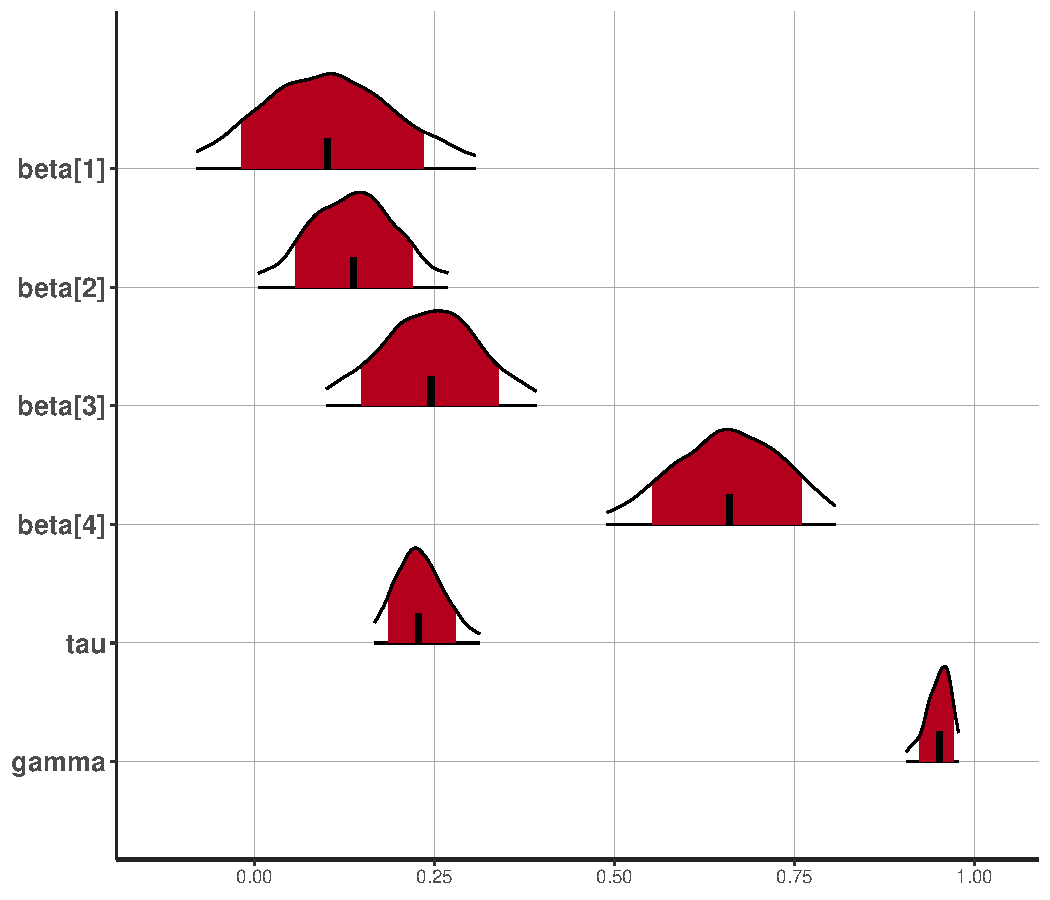
\includegraphics[width=\textwidth]{../figs/mcmc/l_dens.pdf}
        \caption{Estimated posterior of $\beta_2,~\tau_2,~\gamma_2$}\label{fig:denseplot:l}
    \end{subfigure}
    \caption{Estimated posterior using MCMC samples}
    \label{fig:denseplot}
\end{figure}   

\subsection{Prediction}

\autoref{fig:predplot}\은 회귀모형이 예측한 패스트푸드 매장 수의 분포를 나타낸 것이다. 앞의 10개의 패스트푸드 매장 수만을 시각화했으며, 전체 범위는 95\%, 붉은 색은 80\% 신용구간(credible set)을 의미한다. 파란 점으로 실제 $BMK_i$와 $L_i$를 표시하였다. 실제 값과 거의 비슷한 결과를 줌을 확인할 수 있다.
\begin{figure}[!ht]
    \centering
    \begin{subfigure}[b]{0.45\textwidth}
        \centering
        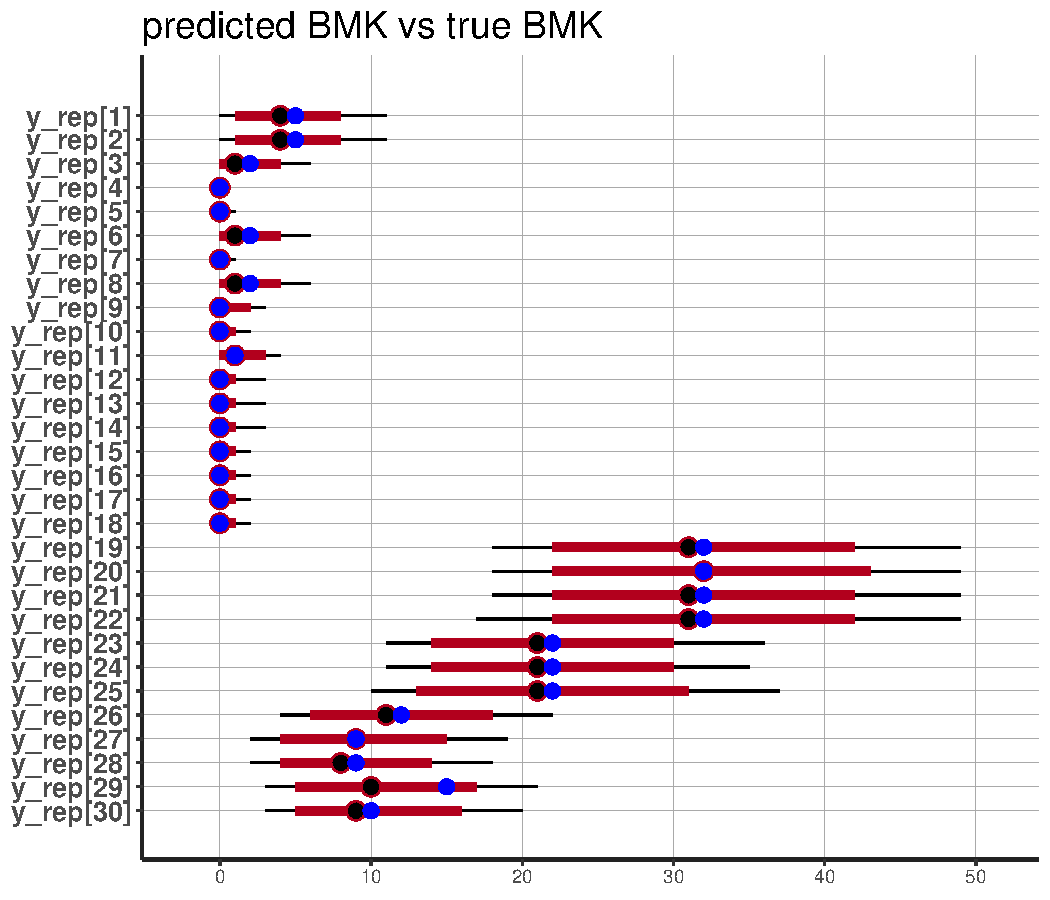
\includegraphics[width=\textwidth]{../figs/mcmc/bmk_pred.pdf}
        \caption{$BMK_i$ 예측치의 분포}\label{fig:predplot:bmk}
    \end{subfigure}
    % \vskip\baselineskip
    \hfill
    \begin{subfigure}[b]{0.45\textwidth}   
        \centering 
        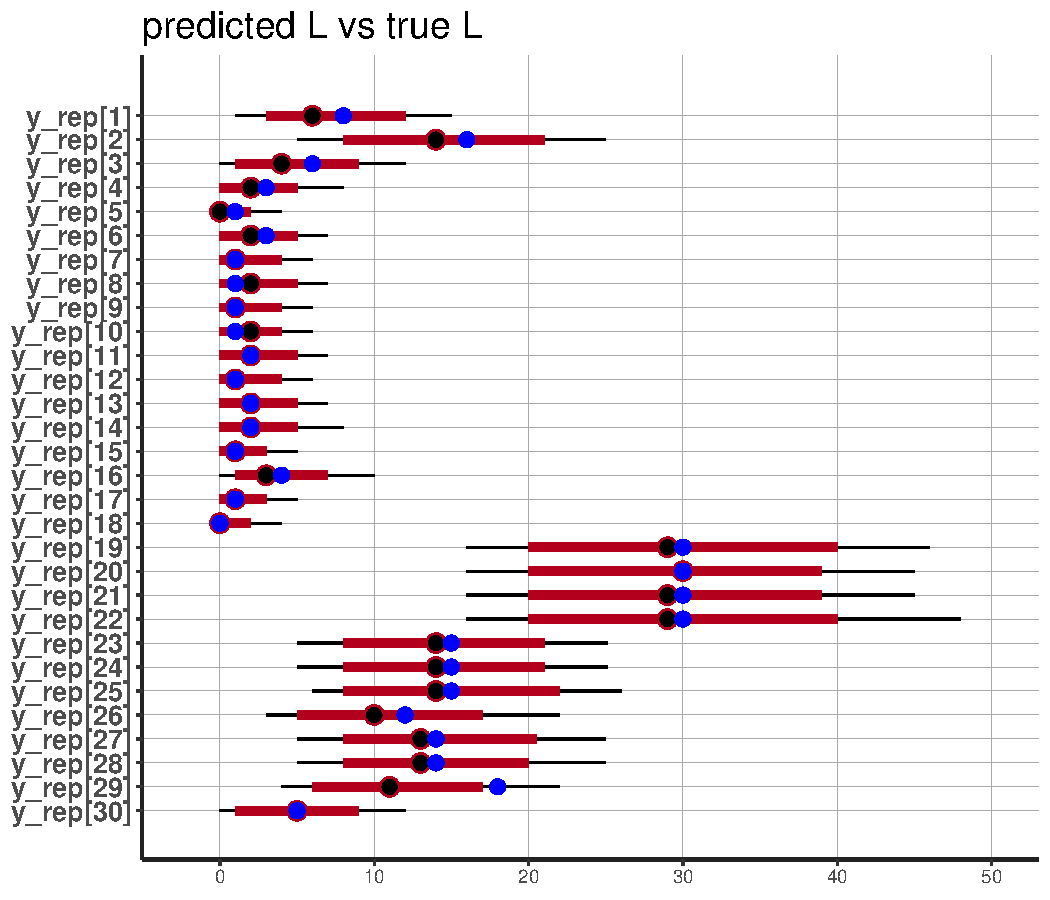
\includegraphics[width=\textwidth]{../figs/mcmc/l_pred.pdf}
        \caption{$L_i$ 예측치의 분포}\label{fig:predplot:l}
    \end{subfigure}
    \caption{패스트푸드 매장 수 예측치의 분포}
    \label{fig:predplot}
\end{figure}   

\autoref{fig:tpredbi}\은 실제 버거지수와 회귀모형으로부터 계산한 버거지수를 나타낸 것이다. 이때, 사후표본 $BNK_{ij},~L_{ij}$로 계산한 버거지수의 추정량 $\hat{BI_i}$\는 비추정량(ratio estimator) 
$$BI_i = \expt{BI_{ij}} = \expt{\frac{BMK_{ij}+1/2}{L_{ij}+1/2}} \approx \frac{\overline{BMK}_i+1/2}{\overline{L}_i+1/2} = \hat{BI_i}$$
\를 사용하였다. 회귀모형이 버거지수를 상당히 잘 예측하고 있는 것을 확인할 수 있다.

\begin{figure}[!ht]
    \centering
    \begin{subfigure}[b]{0.45\textwidth}
        \centering
        \includegraphics[width=\textwidth]{../figs/BI_sig.png}
        \caption{실제 버거지수}\label{fig:truebi}
    \end{subfigure}
    % \vskip\baselineskip
    \hfill
    \begin{subfigure}[b]{0.45\textwidth}   
        \centering 
        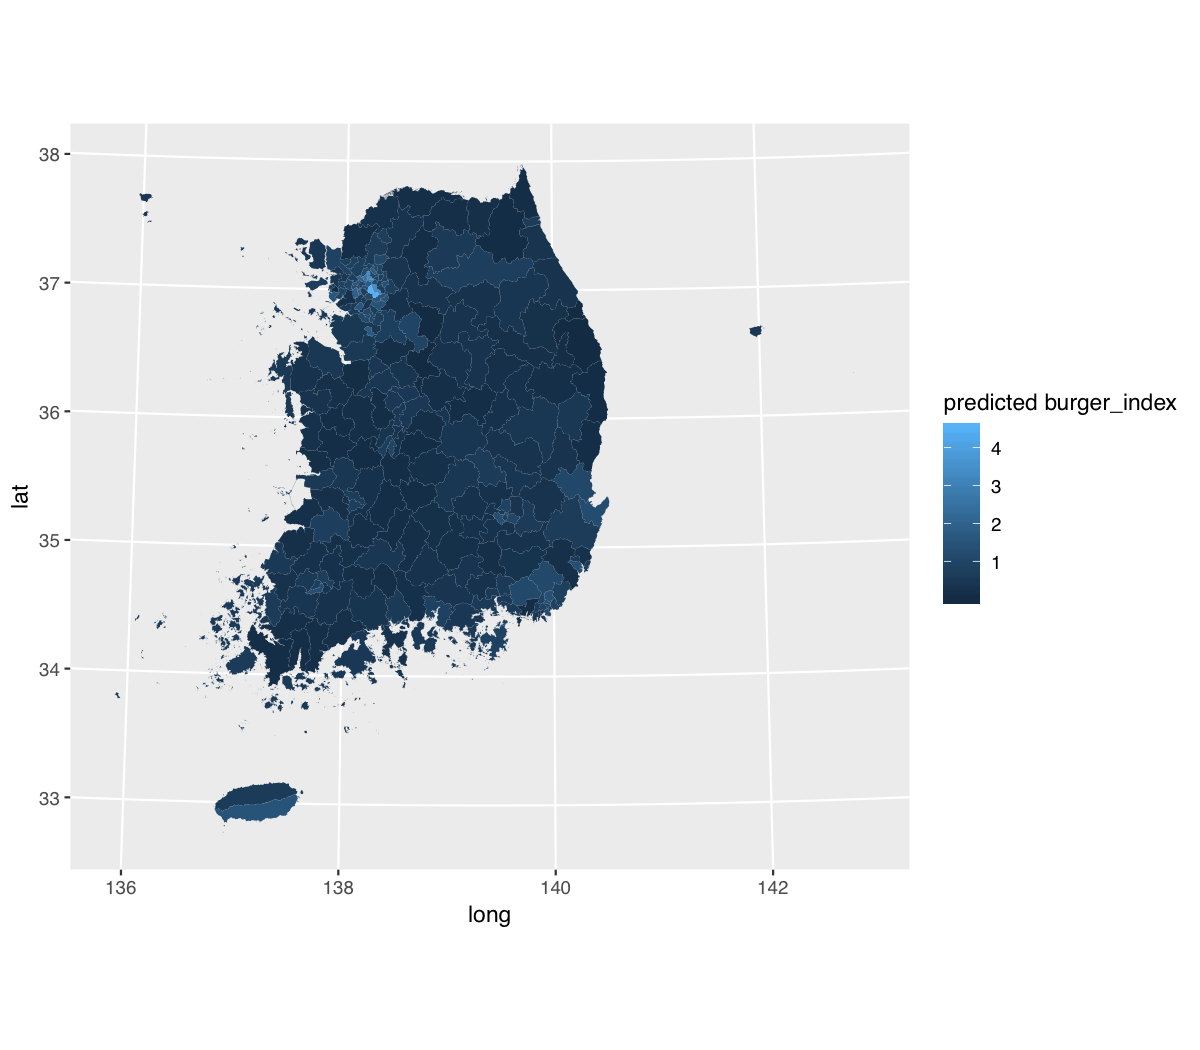
\includegraphics[width=\textwidth]{../figs/pBI_sig.png}
        \caption{회귀모형이 예측한 버거지수}\label{fig:predbi}
    \end{subfigure}
    \caption{버거지수와 예측된 버거지수}
    \label{fig:tpredbi}
\end{figure}   

실제로 \autoref{fig:rebi}와 같이 상대오차 $RE_i = \abs{\hat{BI_i} - BI_i}/BI_i$를 계산하여 그려보면 일부 극단적인 지점을 제외한 곳에서 신뢰할 만한 수준의 예측력을 보임을 확인할 수 있다. 특히, 대도시의 버거지수는 매우 잘 예측된다는 점을 확인할 수 있다. 이는 패스트푸드 매장의 입점 과정에서 상권분석이 고려된다는 사실로 정당화할 수 있다. 또한, 버거지수에서 패스트푸드 매장의 수의 비율을 사용하는 것은 버거지수에 영향을 미치는 다른 요소(면적 등)\을 정규화(normalize)하는 과정으로 이해할 수 있다. 

\autoref{tbl:rebitop5}에는 상대오차가 높은 상위 10개 지점을 정리하였다. 해당 지역들은 모두 버거지수와 예측치가 모두 작아 상대오차가 높게 계산된 것으로 확인된다. 이러한 문제는 비추정량을 사용하여 발생한 것으로 보인다. 또한, 완도군, 울릉군과 같이 인접한 지역이 거의 없는 도서지역에서 예측력이 떨어진다는 점을 확인할 수 있다.

\begin{figure}[!ht]
    \centering
    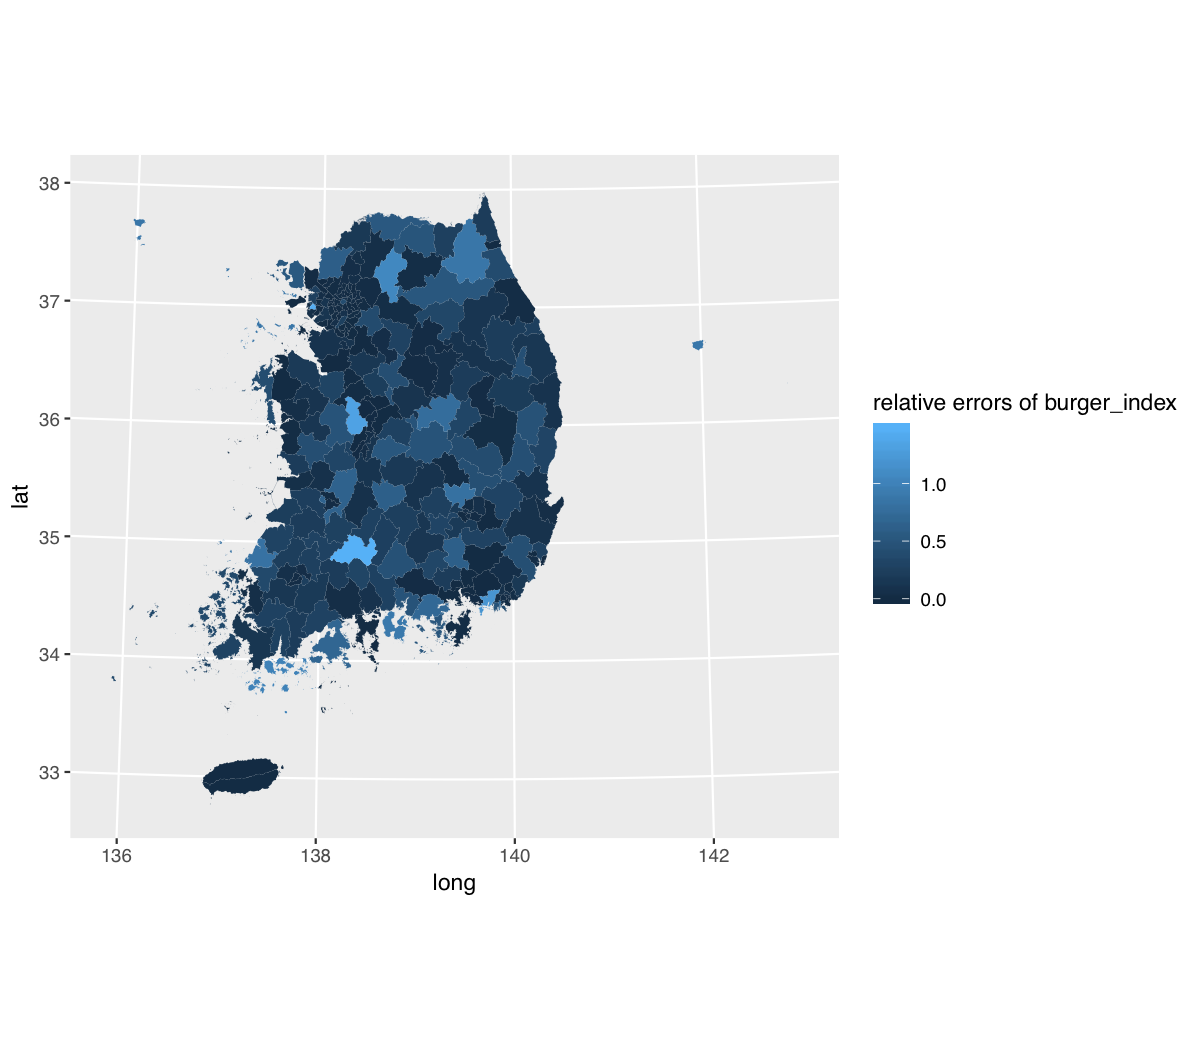
\includegraphics[width=0.7\textwidth]{../figs/reBI_sig.png}
    \caption{버거지수의 상대오차}\label{fig:rebi}
\end{figure}

\begin{table}[ht]
    \centering
    \begin{tabular}{rlrrr}
        \hline
        위치 & $BI_i$ & $\hat{BI_i}$ & $RE_i$ \\ 
        \hline
        남원시 & 0.20 & 0.50 & 1.48 \\ 
        미추홀구 & 0.04 & 0.09 & 1.45 \\ 
        세종특별자치시 & 0.08 & 0.18 & 1.34 \\ 
        강서구 & 0.09 & 0.20 & 1.20 \\ 
        가평군 & 0.11 & 0.23 & 1.06 \\ 
        완도군 & 0.33 & 0.67 & 1.00 \\ 
        남해군 & 0.33 & 0.63 & 0.90 \\ 
        울릉군 & 0.33 & 0.63 & 0.88 \\ 
        옹진군 & 0.33 & 0.62 & 0.87 \\ 
        인제군 & 0.11 & 0.21 & 0.87 \\ 
        \hline
      \end{tabular}
    \caption{상대오차가 높은 상위 10개 시군구}\label{tbl:rebitop5}
\end{table}

\clearpage
\section{Conclusion}\label{sec:con}

본 보고서에서는 다각도로 버거지수를 분석하였다. GIS 자료를 이용해 버거지수를 시각화하였으며 도시 발전도와 상관관계가 있을 것이라 생각되는 인구밀도를 사용하여 공간회귀모형을 적합하였다. 시각화된 버거지수를 통해 기존의 위상구조를 이용한 시각화보다 훨씬 더 현실적인 형태의 분포를 확인할 수 있었으며, 회귀모형으로부터 인구밀도와 버거지수의 구체적인 관계를 확인할 수 있었다. 

보고서의 발전 방향으로 크게 세 가지를 제안한다. 첫째, 더 나은 자료의 사용이 있다. 인접행렬 $W$의 계산 실패와 같은 문제는 정확한 GIS 자료를 사용하여 해결할 수 있을 것으로 생각된다. 예를 들어, 대한민국 통계지리정보 서비스\footnote{\url{https://sgis.kostat.go.kr/view/index}}에서 제공하는 자료를 사용할 수 있다. 자료를 직접 신청해 본 결과, 신청 후 파일을 다운로드 받기까지 약 3일 정도의 시간이 소요되었으며 기존에 사용한 \autoref{tbl:data:description} 자료보다 더 정밀한 형태를 가지고 있음을 확인하였다. 그러나, 자료의 크기와 모형 복잡도 문제로 기존의 자료를 사용해 분석을 진행하였다. 후에 기회가 된다면 통계지리정보서비스에서 다운로드 받은 파일을 이용해 다시 분석을 진행해보고자 한다.

다음으로, 더 나은 공간회귀모형의 적합을 제안한다. 본 보고서에서는 수업시간에 다룬 포아송 모형으로 패스트푸드 매장 수를 추정하고 비추정량을 통해 간접적으로 버거지수를 추정하였다. 반응변수의 분포로 감마분포(gamma distribution), 혹은 절단된 정규분포(truncated normal distribution)\와 같은 분포를 사용한 회귀모형을 사용한다면 버거지수를 직접적으로 추정할 수 있을 것이다. 이러한 접근을 통해 버거지수 추론의 정확도와 해석 면에서 더 나은 결과를 기대할 수 있다.

마지막으로, 인구밀도 외에 도시발전도와 관련된 설명변수들을 사용한 모형의 적합을 제안한다. 대표적으로 도시별 GDP가 있다. 대한민국 통계청에서는 \href{http://kosis.kr/statHtml/statHtml.do?orgId=101&tblId=DT\_2KAA912\_OECD}{OECD 국가의 도시별 GDP}를 제공하고 있으나 시군구별 세분화된 자료를 얻을 수 없어 이번 분석에서는 제외하였다. 이 외에도 도시의 생산량에 영향을 미치는 생산가능인구 비율, 산업 구조 등을 설명변수로 사용한다면 보다 현실적인 모형을 적합할 수 있을 것이다.

\nocite{hoff2009first}
\nocite{lim8}
\nocite{gelman2013bayesian}
\bibliography{refs}

\end{document}